\chapter{Task 1} 
\label{chapter:task1}
In this section a horizontal dipole was simulated with MATLAB. The far field function of the dipole was computed as a function of the angles $\theta$, $\phi$ and excitation current I, which was set to unity. 

We will begin by presenting the theory of the dipole antenna and the far field region in electromagnetic theory. Then we will proceed with presenting the results generated from the MATLAB simulations.  


\section{Theory}
% Far field region
Antenna theory can be greatly simplified be the fact that the fields and different quantities are considered in the far field region only, which is the region where $r > 2D^2/\lambda$. This means that many complicated integrals, Lagrange polynomials, sums  etc. are instead approximated.

Begin by considering the electric field at a point in space $\mathbf{r} = \mathbf{R} + \mathbf{r_0}$ where the origin is set to be $\mathbf{r_0}$ for this coordinate system. The electric field can be considered as a function of $R, \theta, \phi$, i.e. 
\begin{equation}
E(r, \theta, \phi) = E(R, \theta, \phi).
\end{equation}  
and  the far field function times an exponent (which is the electrical field) can be rewritten as 
\begin{align}
\label{elField}
&G( \theta, \phi) \frac{e^{-jkr}}{r} = G'( \theta, \phi) \frac{e^{-jkR}}{R} \approx \\
&\approx G( \theta, \phi) e^{-jk(r-R)}\frac{e^{-jkR}}{R} =  G( \theta, \phi) e^{-jk(\mathbf{r}_o\cdot \hat{r})}\frac{e^{-jkR}}{R}
\end{align}  
where R is the distance $|\mathbf{r} - \mathbf{r}_0|$. In order to do the steps the Fraunhofer approximations in the far field were used,
\begin{equation}
\begin{cases}
& \frac{1}{r} \approx \frac{1}{R} \\
& r \approx R + \mathbf{r}_0\cdot \hat{r}.
\end{cases}
\end{equation}
It is the obvious that the far field can be written as
\begin{equation}
\mathbf{G}_A(\theta, \phi) = \mathbf{G}(\theta, \phi)e^{jk\mathbf{r}_A\cdot \hat{r}} 
\end{equation}
in a space position $\mathbf{r}_A$.
% Mor thoery? !

% Dipole
Consider now a dipole which has a $\hat{I}$ direction, a corresponding current density to this dipole will be 
\begin{equation}
\mathbf{J}_l(l')= I_0 j(l')\hat{I}
\end{equation}
where $I_0$ is the magnitude of the current and j is set to 
\begin{equation}
j(l) = \frac{sin\left(k\left( \frac{l}{2}- |z'|\right)\right)}{sin(kl/2)}.
\end{equation}
The electric field for a dipole may be written as a 
\begin{equation}
\mathbf{E}_d (\hat{r})= \frac{e^{-jkr}}{r}\mathbf{G}_d(\hat{r})
\end{equation}
which is a similar to to equation \eqref{elField} but with a far field which can be written as 
\begin{equation}
\begin{cases}
&  {G}_d(\hat{r}) = \eta I_0C_k[\hat{I}-(\hat{I}\cdot \hat{r})\cdot\hat{r} ]\hat{j}(l\hat{I}\cdot\hat{r}) \\
& \hat{j} = \int_{-l/2}^{l/2}j(l')e^{klj'\hat{I}\cdot\hat{r}} \approx l/2 \text{  if short dipole}
\end{cases}
\end{equation}
% More explination..?!

%Horizontal dipole
Consider finally a horizontal dipole, which is  a dipole with its direction in the y direction. This gives the expressions 
\begin{align}
& \hat{I} = \hat{y} \\
& \hat{I} \cdot \hat{r} = sin\theta sin\phi \\ \label{IrRes}
& \hat{I} -(\hat{I} \cdot \hat{r})\hat{r} = cos\theta sin\phi \hat{\theta} + cos\phi \hat{\phi}. 
\end{align}
The equations above can be understood be considering the spherical coordinates 
\begin{equation}
\begin{cases}
&\hat{x} = sin\theta cos\phi \hat{\theta} + cos\theta cos\phi \hat{\phi} - sin\theta \hat{r} \\
&\hat{y} = sin\theta sin\phi \hat{\theta} + cos\theta sin\phi \hat{\phi} - sin\phi \hat{r} \\
&\hat{z} = -sin\theta  \hat{\theta} - cos\theta \hat{r},
\end{cases}
\end{equation}
It can easily be seen that \eqref{IrRes} indeed holds.



The far field function  for a dipole of length l, sitting at height h can then be written as 
\begin{align}
&\mathbf{G}(\theta, \phi) = C_k\eta I_0 \hat{j}(k\hat{I} \cdot \hat{r})(cos\theta sin\phi \hat{\theta} + cos\phi \hat{\phi} )(e^{jkhcos\theta} -e^{-jkhcos\theta}) \\
& \approx C_k\eta I_0 \hat{j}(k\hat{I} \cdot \hat{r})(cos\theta sin\phi \hat{\theta} + cos\phi \hat{\phi} )(sin(khcos(\theta))). \\
\end{align}
If the dipole is considered to be short  $\hat{j} \approx l/2 $, so the far field function can be described according to  
\begin{equation}
\mathbf{G}(\theta, \phi) = G_{\theta}\hat{\theta} + G_{\phi}\hat{\phi},
\end{equation}
where the $\theta$ and $\phi$ parts of $\mathbf{G}$ are given by the expression

\begin{equation}
G_{\theta} = G_{\theta}(\theta, \phi) = Acos(\theta)sin(\phi)2jsin(khcos(\theta)))
\end{equation}
and 
\begin{equation}
G_{\phi} = G_{\phi}(\theta, \phi) = Acos(\phi)2jsin(khcos(\theta))).
\end{equation} 
The constant A is defined as 
\begin{equation}
A = C_k\eta I_0 l/2
\end{equation} 
with 
\begin{equation}
\begin{cases}
& C_k = -jk/4\pi \\
& \eta \approx 120 \pi [\Omega] \\
& k = \frac{2*pi}{\lambda} \\
& h = \frac{\lambda}{4}\\
& I_0 = \text{incident current}
 \end{cases}
\end{equation}\cite{kildal2000foundations}

\section{Results}
The code for task 1 can be viewed in appendix \ref{section:task1.m}, where the length of the dipole was chosen to be 0.1 $\lambda$ and I to be 1 A in order to get numerical results. 

The $\theta$ part of the far field function can be viewed in figure \ref{task1:Gth} as a function of the angles $\theta$ and $\phi$. 

\begin{figure}[h]
\centering
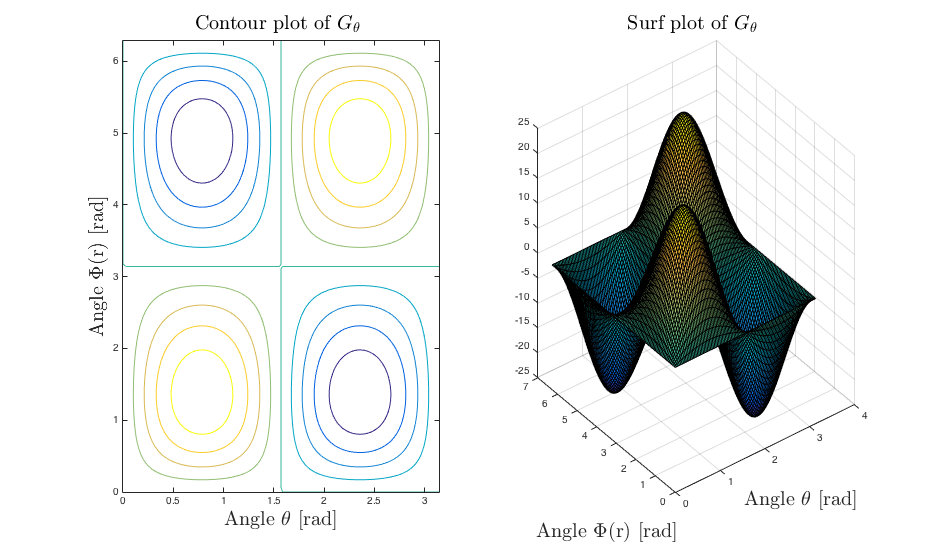
\includegraphics[scale=0.4]{/Users/marikasvensson/Documents/MATLAB/MicroProject/finished/task1/Gth.png}
\caption{This figure shows $G_\theta$ as a function of $\theta$ and $\phi$}
\label{task1:Gth}
\end{figure}


The $\phi$ part of the far field function can be viewed in figure \ref{task1:Gphi} as a function of the angles $\theta$ and $\phi$.


\begin{figure}[h]
\centering
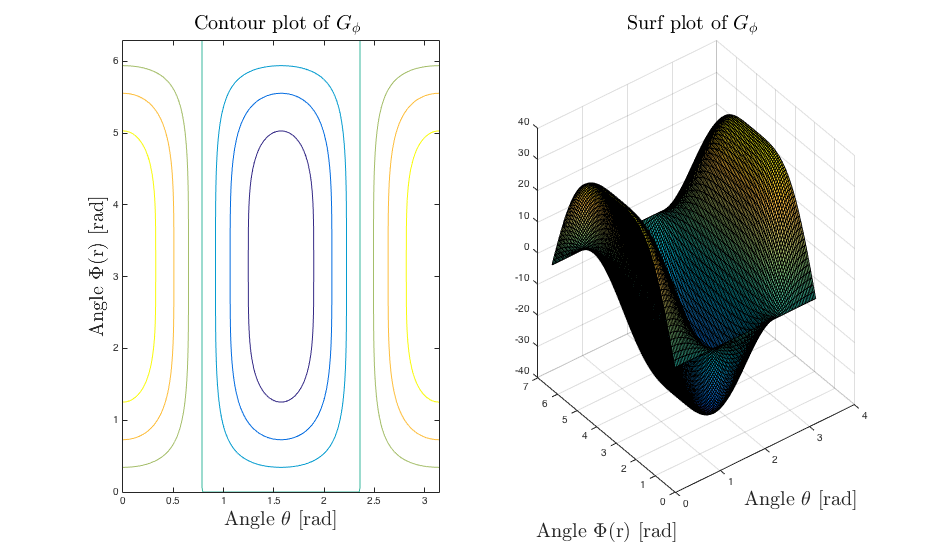
\includegraphics[scale=0.4]{/Users/marikasvensson/Documents/MATLAB/MicroProject/finished/task1/Gphi.png}
\caption{This figure shows $G_\phi$ as a function of $\theta$ and $\phi$}
\label{task1:Gphi}
\end{figure}



